%=========================================
% 	   Einleitung     		 =
%=========================================

\chapter{RSP Versuch}
\section{Allgemeine Beschreibung des Versuchs}
%Kurze Einleitung ins Thema
Im folgenden Kapitel besch�ftigen wir uns mit der Konfiguration eines Switch und einem Router von CISCO. Dazu werden wir einen Switch und einen Router an einen Rechner anschliesen und diese dann �ber eine Konsole konfigurieren. Dar�ber hinaus werden wir uns mit der Software Packet Tracer besch�ftigen. Mit Packet Tracer lassen sich verschiedene Hardware-Szenarien nach spielen und virtuell aufbauen. Es stehen verschiedene Hardware-Produkte zur Verf�gung die sich konfigurieren lassen und beliebig verkabeln lassen.
\section{Switch und Router Konfiguration}
%alles zum Downlink
\subsection{Router start up running config}



\section{Packet Tracer}
Das Folgende Szenario soll erstellt und damit gearbeitet werden. 
\begin{figure}[h]
  \centering
  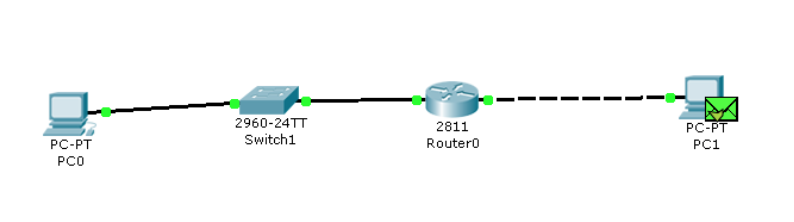
\includegraphics[width=1\textwidth]{tkinhalt/rsp/packettracer/versuchsaufbau.png}
  \caption{SMS von Netzwerk an Mobilestation}
  \label{fig:sms2}
\end{figure}


\subsection{Versuchsaufbau}

\subsection{Messungen}

\subsection{Simmulation Echo-Request/-Reply}

%alles zu ARFCN

\section{Untersuchung des Paketflusses mit Wireshark}

